 %%%%%%%%% %%%%%%%%% %%%%%%%%% %%%%%%%%% %%%%%%%%% %%%%%%%%% %%%%%%%%%

\chapter{Introduzione}


Gli stimoli meccanici rivestono nell'ambito dei sistemi biologici un
ruolo importante nel determinare il corretto funzionamento di cellule,
tessuti e organismi complessi.

Mentre tradizionalmente la biologia si è occupata di studiare come
processi cellulari e inter-cellulari fossero regolati dallo scambio
di molecole biologiche, il ruolo degli stimoli meccanici è stato a
lungo ritenuto marginale nella descrizione di questi processi.

Lo sviluppo di tecniche sempre più avanzate e precise per la
visualizzazione e la manipolazione di molecole all'interno di campioni
biologici ha iniziato a mutare questa concezione: oggi possiamo
indagare nel dettaglio il funzionamento dei motori molecolari
all'interno delle nostre cellule o misurare come variazioni nella
tensione applicata a un polimero possano indurre una riorganizzazione
strutturale nello stesso e cambiarne le proprietà biochimiche.

Per molti processi biologici il ruolo della forza è fondamentale,
ad esempio nei complessi proteici che legano tra di loro le cellule
in un tessuto, le \emph{giunzioni cellulari}.
Queste si comportano come complesse macchine in grado di elaborare
stimoli di tipo biochimico e meccanico, comunicando e interferendo
con le funzioni del resto della cellula.
Esistono diversi tipi di giunzioni cellulari, responsabili di
specifiche funzioni e caratterizzate dalla reciproca interazione di
diversi tipi di proteine. La dinamica della loro interazione viene
modificata e modulata dalle sollecitazioni meccaniche esterne,
permettendo alle giunzioni di comportarsi come \emph{trasduttori}
di segnali meccanici.

Diversi metodi sono stati proposti e realizzati sperimentalmente
per osservare l'attività di meccano-trasduzione nei sistemi
biologici \cite{??}, sfruttando tecniche sia \textit{in vivo} che
\textit{in vitro}, osservando sia gli effetti macroscopici che
le interazioni tra singole molecole.
Nonostante ciò, per quanto riguarda le giunzioni cellulari, siamo
ancora lontani da una descrizione soddisfacente, sia da un punto
di vista qualitativo che quantitativo, dei meccanismi e delle
interazioni coinvolte.

Raggiungere una migliore comprensione riguardo al ruolo e al
funzionamento della meccano-trasduzione nelle giunzioni cellulari
rappresenta un terreno fertile e un forte stimolo per la ricerca
di base interdisciplinare, spingendo scienziati con formazioni diverse
ad unire le loro competenze e sviluppare tecniche complementari, in
modo da acquisire una visione sempre più globale su fenomeni
estremamente complessi, che coinvolgono simultaneamente processi
meccanici, termodinamici e biochimici.

Lo scopo di questo lavoro di tesi è, sviluppare, in gran parte
\textit{ex-novo}, un apparato sperimentale per lo studio della
meccano-trasduzione in contesti complessi come quello delle giunzioni
cellulari, basato sulla manipolazione ottica di due proteine
interagenti e il \textit{tracking} simultaneo, tramite microscopia di
fluorescenza, di altre singole biomolecole nei pressi del sito di
interazione.

La manipolazione tramite pinzette ottiche rappresenta infatti una
strada molto promettente per lo studio, anche quantitativo, di
effetti meccano-biologici, grazie alla possibilità di ottenere una
precisione di posizionamento nanometrica e di applicare alle molecole
un ampio intervallo di forze nell'ordine dei piconewton e dei
femtonewton.

Le pinzette ottiche permettono di sondare il comportamento di
complessi proteici sottoponendo due molecole interagenti a stress
meccanici controllati e andando a osservare come la dinamica delle
interazioni dipenda dalle forze esterne.

Questo tipo di esperimenti si riconduce alle
\emph{spettroscopie di forza},
che in generale vengono realizzate utilizzando diverse tecniche, come
la microscopia a forza atomica, le onde acustiche o le pinzette
ottiche.
I brevissimi tempi di risposta ottenibili utilizzando queste ultime,
inferiori al millisecondo, hanno fatto si che le pinzette ottiche
fossero applicate con successo allo studio di sistemi interagenti con
affinità molto deboli o rapide modifiche conformazionali, come i
motori molecolari \cite{Capitanio2012}.

L'apparato sperimentale descritto in questo lavoro consiste
sostanzialmente in una ricostruzione di quello utilizzato in
\cite{Capitanio2012}
per lo studio dei motori molecolari per quanto riguarda la componente
di spettroscopia di forza, integrato con un sistema di microscopia di
fluorescenza che consenta di osservare simultaneamente la dinamica di
singole molecole interagenti con le proteine intrappolate.

Infatti, fino a ora il principale limite di questi esperimenti è
stato quello di produrre informazioni dinamiche
esclusivamente sui due componenti interagenti selezionati per la
spettroscopia di forza, trascurando ogni altra possibile interazione.
Se in diversi scenari questo è più che sufficiente, alcuni
sistemi biologici, questo approccio mostra evidenti limiti nello
studio di una complessa rete di interazioni come quella delle
giunzioni cellulari.

Un apparato con queste caratteristiche dovrebbe consentire,
durante un esperimento di spettroscopia di forza, di registrare
simultaneamente sia la risposta meccanica delle due proteine
immobilizzare, sia l'eventuale interazione con altri fattori
opportunamente marcati presenti nella soluzione usata per
l'esperimento.

L'ostacolo principale al raggiungimento di questo risultato è dato
dalla difficoltà di visualizzare, tramite microscopia ottica,
l'attività di una singola molecola fluorescente sopra un fondo di
fluorofori liberi in soluzione.

Una soluzione tipicamente adottata prevede l'uso di schemi di
illuminazione come la riflessione interna totale
(TIRF, \textit{Total Internal Reflection Fluorescence microscopy})
o i fogli di luce inclinati
(HILO, \textit{Highly Inclined and Laminated Optical sheet
microscopy}),
in modo da ridurre il volume di campione eccitato e quindi l'emissione
di fluorescenza di fondo.

Questi schemi di illuminazione però richiedono requisiti molto
stringenti.
Ad esempio per poter utilizzare la TIRF, come approfondito in sezione
\ref{sec:fluo} è necessario che il volume osservato sia nelle
immediate vicinanze della superficie del vetrino
coprioggetti usato per la preparazione del campione,
condizione che è impossibile realizzare negli esperimenti di
spettroscopia di forza, dove le proteine vengono funzionalizzate su
sfere dielettriche di dimensioni micrometriche.
In questo caso infatti il volume di campione
dove si trovano le proteine interagenti ha uno quota significativa
(diverse centinaia di micrometri) rispetto al vetrino coprioggetti.

Scopo dell'apparato sperimentale sarà anche studiare la possibilità di
superare questo limite usando la sfera dielettrica come risuonatore
ottico, e quindi come strumento in grado di trasferire la radiazione
di eccitazione dall'immediata prossimità del vetrino coprioggetti ai
fluorofori presenti in prossimità del sito di interazione.
In questo modo il segnale proveniente da molecole fuori fuoco,
lontane dalla microsfera, sarebbe efficacemente soppresso.

Nelle prossime sezioni è possibile trovare una trattazione più
approfondita degli argomenti introdotti, in particolare nella sezione
\ref{sec:giunzioni} vengono introdotte due importanti tipologie di
giunzioni cellulari particolarmente interessanti per studio con un
sistema combinato come quello qui descritto.\\
Nella sezione \ref{sec:ot} vengono trattate in maniera più
approfondita le pinzette ottiche e la loro applicazione agli
esperimenti di spettroscopia di forza.\\
Nella sezione \ref{sec:fluo} vengono introdotti i principali limiti
della microscopia di fluorescenza e le soluzioni proposte per il loro
superamento.

Nel capitolo \ref{cap:methods} vengono descritte nel dettaglio le
caratteristiche dell'apparato sperimentale realizzato e le procedure
di validazione, calibrazione e acquisizione dei dati.

Nel capitolo \ref{cap:results} sono analizzati i dati prodotti durante
le operazioni di validazione dell'apparato sperimentale e delle
procedure di misura per valutare le prestazioni ottenibili e la loro
adeguatezza agli esperimenti ipotizzati.


% Introduction on the importance of mechanotransduction



 %%%%%%%%% %%%%%%%%% %%%%%%%%% %%%%%%%%% %%%%%%%%% %%%%%%%%% %%%%%%%%%



% between 

\section{Giunzioni cellulari}
\label{sec:giunzioni}

Le giunzioni cellulari svolgono un ruolo fondamentale per l'esistenza
stessa degli organismi multicellulari.
Esse sono infatti responsabili della capacità delle cellule di
connettersi l'una con l'altra e di organizzarsi per formare tessuti e
organi con funzioni specifiche.
Le funzioni delle giunzioni cellulari vanno ben oltre quelle di una
passiva struttura di raccordo: esse sono responsabili, ad esempio,
di veicolare informazioni e sostanze tra una cellula e l'altra,
guidare la loro proliferazione o migrazione, mantenere la stabilità
dei tessuti o avviarne la riparazione quando necessario.

\begin{figure}[ht]
    \centering
    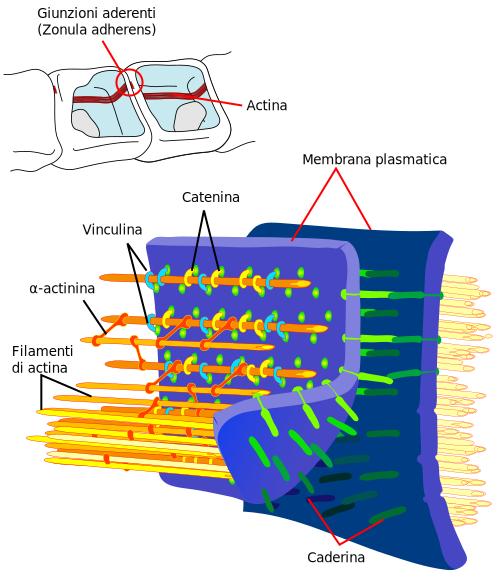
\includegraphics[width=0.5\linewidth]{images/adjunc.pdf}
    \caption{Sequenza di cellule connesse da \emph{giunzioni aderenti}
        (sopra) e dettaglio di una giunzione aderente, con indicazione
        delle principali proteine coinvolte (sotto)}
    \label{fig:ad_jun}
\end{figure}

Le giunzioni cellulari possono connettersi direttamente a strutture
interne della cellula (come il citoscheletro) e si formano
dall'auto-assemblamento di un grande numero di proteine differenti.
Per loro natura attraversano la membrana cellulare andando a formare
legami con strutture analoghe presenti in cellule adiacenti o con
strutture intermedie di supporto, come la matrice extra-cellulare.

Esistono diversi tipi di giunzioni che svolgono funzioni specifiche.
Un tipo di giunzione molto comune nei tessuti epiteliali e 
endoteliali è la \emph{giunzione aderente}, rappresentata in modo
schematico in figura \ref{fig:ad_jun}.

Nelle giunzioni aderenti la proteina che direttamente ancora il
complesso alla membrana plasmatica è la \emph{caderina}.
Questa è una proteina trans-membrana costituita da un dominio di coda
citoplasmatico e un dominio di testa esterno alla membrana cellulare.
Il dominio extra-membrana è in grado di dimerizzare con domini
analoghi presenti in cellule adiacenti, formando la giunzione.
Il dominio intra-membrana permette di stabilire un collegamento
diretto tra la giunzione cellulare e il citoscheletro di actina,
grazie al legame con una classe di proteine, le \emph{catenine},
in grado di legarsi sia con la coda della caderina che con i filamenti
di actina del citoscheletro.

Oltre a questa connessione diretta esistono altre proteine che
mantengono una connessione indiretta, legando ad esempio le catenine
con il citoscheletro. É stato scoperto \cite{??} che le proteine
\emph{vinculina} e \emph{$\alpha$-actinina} svolgono questa attività.

Sebbene la funzione di questi collegamenti indiretti non sia stata
ancora del tutto compresa, è stato dimostrato che la sua presenza
delle proteine responsabili è fondamentale per il corretto sviluppo
dei tessuti.
Esperimenti su colture cellulari in il gene che codifica l'espressione
della vinculina è stato rimosso suggeriscono come, oltre ad una
riduzione generale dell'adesione tra cellule, si perda alcune funzioni
di regolazione
e modulazione dell'attività delle giunzioni.

La vinculina, quindi, così come altre proteine secondarie, potrebbe
avere un ruolo nel modulare i meccanismi di adesione e svolgere un
ruolo nei processi di meccano-trasduzione.

La possibilità di realizzare esperimenti di spettroscopia di forza in
cui è possibile tenere traccia dell'attività di una o più proteine
secondarie apre la strada verso una maggiore comprensione del loro
ruolo.

Lo stato attuale delle conoscenze sulla rete di interazioni che
governa e regola il funzionamento delle giunzioni aderenti è riportato
schematicamente in Appendice, sotto forma di diagramma delle vie di
segnalazione.

\begin{figure}[ht]
    \centering
    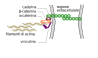
\includegraphics{images/aj.pdf}
    \caption{Ruolo di \textbf{caderina} e catenine nelle
        \textit{giunzioni aderenti}}
    \label{fig:aj}
\end{figure}

\vspace{1em}
Un'altra classe di giunzioni cellulari è rappresentata dalle
giunzioni occludenti (\textit{tight junction}), la cui caratteristica
principale è quella di sigillare lo spazio intercellulare, rendendolo
impermeabile e impedendo a molecole e ioni di attraversare un
tessuto.
L'organizzazione spaziale delle giunzioni occludenti consente inoltre
la creazione di canali selettivamente permeabili per il trasporto
di specifiche molecole, tuttavia ancora non sono chiari i meccanismi
che modulano e regolano il loro funzionamento.
Come nel caso delle giunzioni aderenti questo emerge dall'interazione
tra un certo numero di proteine interagenti.

\begin{figure}[ht]
    \centering
    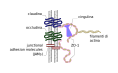
\includegraphics{images/tj.pdf}
    \caption{Ruolo di \textbf{ZO-1} nelle \emph{giunzioni occludenti}}
    \label{fig:tj}
\end{figure}

Diverse proteine attraversano la membrana e dimerizzano
con le loro omologhe appartenenti alla cellula adiacente,
tra le quali \emph{claudina}, \emph{occludina} e diverse
proteine appartenenti alla classe delle \textit{junctional
adhesion molecules}, (JAM).
Queste proteine di membrana si legano alla proteina
\textit{Zona occludens 1}, ZO-1 che, come mostrato da
recenti studi \cite{??}, potrebbe modulare la formazione
delle giunzioni e occuparsi della trasduzione di segnali
meccanici.
Inoltre vi sono evidenze sul ruolo di una terza proteina,
la \textit{cingulina}, nel modulare l'interazione di ZO-1
con il citoscheletro di actina. Un'ipotesi è che il
legame cingulina-ZO-1 possa indurre delle modifiche
conformazionali in ZO-1 tali da consentire un legame
diretto con in filamenti di actina.
Anche in questo caso, per comprendere il ruolo della cingulina
nella trasduzione dei segnali meccanici, sembra promettente
utilizzare una tecnica che consenta, durante l'osservazione
dell'interazione di due proteine sottoposte a stress
meccanici, di osservare l'eventuale attaccamento al complesso
di una terza proteina. Ad esempio sarebbe possibile ipotizzare
un esperimento in cui allo studio dell'effetto delle sollecitazioni
meccaniche sul legame actina-ZO-1 viene aggiunta l'osservazione
dell'attività della cingulina attraverso microscopia di fluorescenza.



\section{Manipolazione ottica di molecole biologiche}
\label{sec:ot}

Le pinzette ottiche (o \textit{optical tweezers}, OT) sono strumenti
che sfruttano la \emph{forza di radiazione} esercitata da un fascio
laser gaussiano altamente focalizzato su materiali dielettrici, in
modo da intrappolare e manipolare oggetti microscopici con una
precisione sub-nanometrica.

Questa tecnologia sfrutta il gradiente d'intensità di un fascio
gaussiano focalizzato interagente con particelle dielettriche immerse
in un fluido. L'interazione delle particelle con la radiazione fa si
che queste risentano di una forza di richiamo verso una posizione
di equilibrio in prossimità del fuoco del fascio.

Fin dalla loro ideazione vennero subito messe in luce le potenzialità
di questa tecnica quando applicata alla manipolazione di campioni
biologici.

Arthur Ashkin fu, nel 1986, il primo a realizzare sperimentalmente
delle pinzette ottiche, riuscendo a intrappolare microsfere sintetiche
e batteri\cite{Ashkin:86}. Per questo risultato gli fu conferito il
premio Nobel nel 2018, \emph{``per le pinzette ottiche e le loro
applicazioni ai sistemi biologici''}.

Grazie alle pinzette ottiche è possibile intrappolare solidi
dielettrici di diversa dimensione e natura.
Per ottenere la capacità di manipolare individualmente singole
molecole, come le proteine non è possibile procedere ad un
intrappolamento diretto.

Si rende necessario quindi sviluppare protocolli per funzionalizzare
la superficie di sfere dielettriche e legarci le molecole che
intendiamo studiare.

Tipicamente esperimenti di questo tipo vengono realizzati utilizzando
sfere dielettriche di dimensioni micrometriche funzionalizzate legando
covalentemente molecole di \textit{streptavidina} alla loro
superificie.

In questo modo è possibile successivamente ottenere il legame delle
microsfere col polimero biologico d'interesse, purché esso sia stato
preventivamente biotilinato. Si sfrutta in questo modo il legame 
streptavidina-biotina, estremamente stabile e praticamente
irreversibile (vedi figura \ref{fig:biotin-streptavidin}).

\begin{figure}[ht]
    \centering
    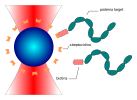
\includegraphics[width=0.5\linewidth]{images/biotin-streptavidin.pdf}
    \caption{Manipolazione di una proteina target utilizzando una
        microsfera intrappolata e il legame biotina-streptavidina.}
    \label{fig:biotin-streptavidin}
\end{figure}

Per descrivere quantitativamente il funzionamento delle pinzette
ottiche consideriamo in generale l'effetto dell'interazione tra
una microsfera dielettrica, immersa in una soluzione liquida, e
la radiazione elettromagnetica prodotta da un fascio laser gaussiano
focalizzato.

In generale la forza a cui è soggetta la microsfera interagente
col campo elettromagnetico può essere scomposta in due contributi:

\begin{itemize}
    \item La \textbf{forza di \textit{scattering}} o pressione di
        radiazione, sempre orientata nella direzione di propagazione
        della radiazione e proporzionale alla sua intesità.
    \item La \textbf{forza di dipolo} o gradiente, proporzionale
        al gradiente d'intensità della radiazione elettromagnetico.
\end{itemize}

L'origine di questi due contributi e la dipenza dalle caratteristiche
della microsfera e del liquido utilizzati possono essere derivate
analiticamente dalle equazioni di Maxwell nei limiti del regime
di Rayleigh, ovvero quando le dimensioni della sfera sono molto
inferiori alla lunghezza d'onda della radiazione utilizzata.

In questo limite possiamo considerare il materiale interagente con la
radiazione come un dipolo elettrico puntiforme, associato ad una
polarizzabilità $\alpha$. Il vettore di polarizzazione nel dipolo
puntiforme sarà quindi $\vec{p} = \alpha \vec{E}$.

La pressione di radiazione sarà quindi proporzionale all'impulso
dei fotoni retrodiffusi per \textit{scattering} Rayleigh.
Nel caso di una microsfera di raggio $a$, indice di rifrazione $n$,
immersa in un fluido con indice di rifrazione $m$, la forza di
\textit{scattering} può essere espressa\cite{HARADA1996529} come:

\begin{equation}
\vec{F}_r = \hat{k} \frac{8 \pi n k^4 a^6}{3c}
\left(
\frac{(n/m)^2 - 1}{(n/m)^2 + 2}
\right)^2
\end{equation}

L'espressione della forza gradiente può essere ottenuta
dall'interazione lorentziana tra la radiazione e il dipolo puntiforme:

$$ \vec{F}_g =
    \left(
        \vec{p} \cdot \vec{\nabla}
    \right)
    \vec{E}
    + \frac{d\vec{p}}{dt} \times \vec{B}
$$

Ovvero, una volta sostituito il vettore di polarizzazione:

$$ \vec{F}_g =
    \alpha
    \left[
        \left( \vec{E} \cdot \vec{\nabla} \right) \vec{E}
        + \frac{d\vec{E}}{dt} \times \vec{B}
    \right]
$$

E infine, tenendo conto delle \emph{equazioni di Maxwell} e
dell'algebra dei vettori:

\begin{equation}
\label{dipole_force}
\vec{F_g} =
    \alpha 
    \left[
        \frac{1}{2}\nabla E^2
        + \frac{d}{dt}\left(\vec{E} \times \vec{B}\right)
    \right]
\end{equation}

Questa ultima forma (equazione \ref{dipole_force}) ci permette di
mettere in evidenza il termine $\frac{d}{dt}(\vec{E} \times \vec{B})$,
ovvero la derivata temporale di una quantità oscillante molto
rapidamente (\SI{> 1e14}{\Hz}), che
può tranquillamente essere considerata costante se confrontata con in
tempi tipici dell'evoluzione meccanica del sistema.
Il secondo termine può quindi essere trascurato e, sostituendo ad
$\alpha$ l'espressione per la polarizzabilità della microsfera
otteniamo:

\begin{equation}
\vec{F}_g = 
    \frac{2\pi n a^3}{c}
    \left(
        \frac{(n/m)^2 - 1}{(n/m)^2 + 2}
    \right)
    \nabla I(\vec{r})
\end{equation}

Il risultato netto dei due contributi è che la microsfera tenderà ad
occupare una posizione di equilibrio nel punto in cui i due contributi
si cancellano e, se perturbata, risentirà di una forza di richiamo
verso la posizione di equilibrio.

Un risultato qualitativamente identico è dimostrabile nel limite
dell'ottica geometrica, quando la particella è al contrario di
dimensioni molto maggiori alla lunghezza d'onda intermedia.

Il caso intermedio richiede l'uso della più complessa teoria
Lorenz-Mie e spesso il ricorso a soluzioni numeriche, ma l'idea
qualitativa alla base dell'intrappolamento resta valida.

Nel caso generale i requisiti per un intrappolamento efficace sono
quelli di avere una forza di gradiente maggiore di quella di
scattering e una energia cinetica delle particelle intrappolate
sufficientemente bassa (quindi un fluido sufficientemente viscoso).

Per le nostre applicazioni è sufficiente considerare una forza di
richiamo del tipo 

\begin{equation}
    \vec{F} = -k(\vec{x}-\vec{x}_{eq})
\end{equation}

\begin{figure}[ht]
    \centering
    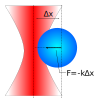
\includegraphics[scale=.4]{images/fkx.pdf}
    \caption{Effetto netto della forza di radiazione}
    \label{fig:fkx}
\end{figure}

Il valore di $k$ per una certa trappola ottica, come vedremo, può
essere determinato attraverso un'apposita procedura di calibrazione
che sfrutta la diffusione della microsfera all'interno della trappola.

Inoltre è necessario considerare l'effetto degli urti con le molecole
della soluzione liquida in cui la sfera è immersa, che hanno i due
seguenti effetti:
\begin{itemize}
    \item La presenza di un attrito viscoso, proporzionale alla
        velocità relativa della sfera rispetto al fluido
    \item La fluttuazione della sfera rispetto alla posizione di
        equilibrio (moto browniano).
\end{itemize}

Grazie alla termodinamica statistica è possibile mettere in relazione
lo spettro delle fluttuazioni di posizione di una sfera intrappolata
con il parametro $k$ della forza elastica di richiamo
(vedi Appendice \ref{app:fluctuaction_spectrum}).
In questo modo, una volta determinato $k$, è possibile mettere
in relazione il valore delle forze esterne agenti sulla sfera con il
suo spostamento dalla posizione di riposo.


\section{Microscopia di fluorescenza di singola molecola}
\label{sec:fluo}

% come evitare ripetizione "singola(e) molecola(e)"
Tipicamente, le tecniche di microscopia di fluorescenza di singola
molecola consentono di sondare la posizione e i movimenti di singole
molecole con risoluzioni spaziali e temporali prossime,
rispettivamente, al nanometro e al millisecondo.

In ambito biologico le molecole che vengono osservate con questa
tecniche sono polimeri di varia natura, come proteine e acidi
nucleici. Anche se alcune di queste molecole possono avere una
debole fluorescenza intrinseca, si fa quasi sempre ricorso alla
marcatura con fluorofori, cioè molecole con caratteristiche di
fluorescenza note e elevata resa quantica. In questo modo è
possibile ottenere livelli di segnale maggiori e soprattutto 
un'elevata specificità nel rendere rilevabili solo le molecole
che presentano caratteristiche di interesse.
Queste due proprietà sono, come vedremo, molto importanti per
raggiungere una buona precisione di localizzazione.

Le tecniche di microscopia di fluorescenza sono molto flessibili
e spesso non distruttive: consentono di osservare processi biologici
in tempo reale in celle di reazione, colture cellulari e organismi
viventi.

Un esperimento di microscopia di fluorescenza generalmente
comprende due fasi principali:
\begin{itemize}
    \item La marcatura delle molecole di interesse, ovvero
        l'attuazione di un protocollo per legare specificamente il
        fluoroforo scelto alle molecole che si intende visualizzare.
    \item La produzione delle immagini, mediante l'illuminazione del
        campione alla lunghezza d'onda di eccitazione del fluoroforo
        e la raccolta della radiazione emessa alla lunghezza d'onda
        di emissione.
\end{itemize}

Per quanto riguarda la marcatura (o \textit{labeling}) delle
molecole esistono svariate strategie e tipologie di fluorofori
utilizzabili. Il fluoroforo può essere legato covalentemente alla
molecola di interesse attraverso apposite reazioni chimiche,
può essere incorporato in un anticorpo, ovvero una proteina
in grado di riconoscere siti specifici di altre molecole e legarvisi
non covalentemente, oppure tramite l'ingegneria genetica è possibile
fornire a delle cellule le istruzioni per sintetizzare e assemblare
proteine contenenti regioni fluorescenti.
I fluorofori utilizzati possono essere piccole molecole organiche,
nanoparticelle realizzate in materiali semiconduttori (come i punti
quantici) oppure sequenze di amminoacidi.
In commercio si trovano numerosi fluorofori operanti in molteplici
regioni dello spettro visibile e con protocolli di marcatura
standardizzati. La scelta del fluoroforo e del protocollo di marcatura
devono tener conto di numerosi fattori, tra i quali: le condizioni
dell'esperimento (in vivo o in vitro), le possibili interferenze col
comportamento del sistema studiato, la compatibilità con le sostanze
chimiche usate in soluzione, la stabilità del fluoroforo stesso e il 
suo tempo di vita.

Per la produzione delle immagini esistono due macro-categorie di
tecniche: le microscopie a campo largo (o \textit{wide-field}) e
le miscroscopie a scansione puntiforme.
Nel primo caso l'intero volume osservato viene illuminato
uniformemente e la radiazione emessa per fluorescenza viene raccolta
e ingrandita da un opportuno cammino ottico che ricostruisce
l'immagine sulla matrice di un sensore CMOS o CCD.
Nel secondo caso l'area di interesse viene suddivisa in un reticolo
tridimensionale di punti e ogni punto viene acquisito sequenzialmente,
illuminando il più piccolo volume circostante possibile e raccogliendo
tutta la radiazione emessa proveniente dal medesimo volume in un
unico punto, coincidente con l'apertura di un fotodiodo o di un
fotomoltiplicatore.

Il principale vantaggio delle tecniche a scansione rispetto a quelle
a campo largo risiede in una più marcata soppressione del
rumore di fondo dovuto all'emissione di fluorescenza fuori dal
piano focale. I microscopi che sfruttano queste tecniche sono infatti
equipaggiati di opportuni accorgimenti per filtrare sia la radiazione
di eccitazione che quella raccolta, in modo da selezionare uno strato
estremamente sottile del volume del campione.
Le dimensioni del volume selezionato per ogni
punto acquisito possono avvicinarsi molto al limite di diffrazione,
in questo modo è possibile visualizzare in maniera estremamente nitida
strutture con dettagli di dimensioni confrontabili con il limite
di diffrazione.
Lo svantaggio principale invece sta nella massima risoluzione
temporale ottenibile: per acquisire un'immagine è necessario
muovere il campione (o il fascio di illuminazione) attraverso
l'intero reticolo e per ogni punto è richiesto un tempo di sosta
adeguato a raccogliere un numero sufficiente di fotoni.
La risoluzione temporale di un microscopio a scansione, quindi,
decresce all'aumentare delle dimensioni dell'area osservata e della
densità di punti acquisita.

La microscopia a campo largo, acquisendo simultaneamente tutto il
fotogramma in una sola volta, consente di raggiungere risoluzioni
temporali molto elevate anche per campioni estesi. La velocità
di acquisizione di un singolo fotogramma è essenzialmente limitata
dalla sensibilità del sensore usato e dalla velocità della sua scheda
elettronica.
Tuttavia, in questo caso, sul sensore si va a sommare all'immagine
proveniente dai fluorofori nel piano focale quella, fuori fuoco,
di tutti gli emettitori che si trovano su piani diversi attraversati
dal fascio.
In campioni con una elevata densità di fluorofori liberi in soluzione
questo effetto viene particolarmente accentuato, con un impatto
negativo sul rapporto segnale/rumore ottenibile e di conseguenza
sulla possibilità di individuare e localizzare singole molecole.

Per ottenere una sensibilità di singola molecola senza sacrificare
la risoluzione temporale sono state sviluppate tecniche che,
manipolando il fascio di eccitazione, consentono di ridurre lo
spessore del volume di campione eccitato, come la microscopia a
riflessione interna totale
(TIRF, \textit{Total Internal Reflection Fluorescence microscopy})
o quella a fogli di luce inclinati
(HILO, \textit{Highly Inclined and Laminated Optical sheet
microscopy}).
Grazie a queste due tecniche è possibile ottenere una sensibilità
di singola molecola a una risoluzione temporale nell'ordine dei
millisecondi, rendendo possibile ad esempio il tracciamento
degli spostamenti di una proteina.

\subsection{TIRF}


